\section{Comparison of Coordinator and Probe Accuracy}
\label{sec:ch8-overview}

\phantomsection\label{rq:ch8-rq1-intro}
\begin{rqbox}[RQ1]
On requests where the correct sub-agent is difficult to determine from the wording alone, does a probe on the hidden states of a coordinator model recover the correct sub-agent more accurately than the coordinator's own selection?
\end{rqbox}


\noindent To answer \hyperref[rq:ch8-rq1-intro]{\textbf{RQ1}}, this section compares the accuracy of the probe with the accuracy of the coordinator on both datasets and on each difficulty tier. The comparison across the difficulty tiers shows how the accuracy of the probe changes against the accuracy of the coordinator as the difficulty increases. The comparison between the two datasets shows how the multi-turn setting affects the accuracy.

The correct sub-agent is difficult to determine from the wording alone when text-only classifiers reach a low accuracy on the request (Section~\ref{subsec:lexical-separability}). The difficulty tiers lower this accuracy from \texttt{plain} to \texttt{adversarial} (Section~\ref{sec:dataset-baselines}).

\subsection{Accuracy on the Whole Dataset}
\label{subsec:ch8-overview-all}

Table~\ref{tab:ch8-overview} reports, from Section~\ref{sec:ch7-results}, the AUC macro of the probe, the accuracy of the coordinator and of the probe, their difference, and the McNemar test between the two, Holm-corrected as in Chapter~\ref{chap:probing-results}. The \emph{margin} $\Delta$ is the difference between the two accuracies, computed as the accuracy of the probe minus the accuracy of the coordinator.

\begin{table}[htbp]
    \centering
    \small
    \setlength{\tabcolsep}{4pt}
        \begin{tabular}{@{}lccccc@{}}
            \toprule
            \textbf{Model} & \textbf{\begin{tabular}[b]{@{}c@{}}probe\\AUC macro\end{tabular}} & \textbf{\begin{tabular}[b]{@{}c@{}}coordinator\\accuracy\end{tabular}} & \textbf{\begin{tabular}[b]{@{}c@{}}probe\\accuracy\end{tabular}} & $\boldsymbol{\Delta}$ & $\boldsymbol{p_{\text{holm}}}$ \\
            \midrule
            \multicolumn{6}{@{}l}{\textit{Single-turn}} \\
            \midrule
            \texttt{gemma4-e2b-it} & 0.976 & \worst{0.736} & 0.848 & \rgain{0.112} & $<10^{-4}$ \\
            \texttt{qwen3-4b} & 0.977 & 0.752 & 0.864 & \rgain{0.112} & $<10^{-4}$ \\
            \texttt{qwen3-8b} & 0.974 & 0.772 & \worst{0.845} & \rgain{0.073} & $<10^{-4}$ \\
            \texttt{gemma4-12b-it} & 0.988 & 0.873 & 0.916 & \rgain{0.043} & $<10^{-4}$ \\
            \texttt{gemma4-26b-a4b-it} & 0.989 & \best{0.888} & \best{0.921} & \rgain{0.033} & 0.00012 \\
            \texttt{llama3.3-70b} & 0.985 & 0.770 & 0.894 & \rgain{0.124} & $<10^{-4}$ \\
            \texttt{qwen2.5-72b} & 0.988 & 0.761 & 0.907 & \rgain{0.146} & $<10^{-4}$ \\
            \midrule
            \multicolumn{6}{@{}l}{\textit{Multi-turn}} \\
            \midrule
            \texttt{gemma4-e2b-it} & 0.947 & \worst{0.702} & 0.782 & \rgain{0.080} & $<10^{-4}$ \\
            \texttt{qwen3-4b} & 0.959 & 0.745 & 0.814 & \rgain{0.069} & $<10^{-4}$ \\
            \texttt{qwen3-8b} & 0.928 & 0.738 & \worst{0.744} & \rgain{0.006} & \pns{0.65} \\
            \texttt{gemma4-12b-it} & 0.979 & 0.855 & \best{0.879} & \rgain{0.024} & 0.011 \\
            \texttt{gemma4-26b-a4b-it} & 0.977 & \best{0.856} & 0.878 & \rgain{0.022} & 0.024 \\
            \texttt{llama3.3-70b} & 0.950 & 0.736 & 0.810 & \rgain{0.074} & $<10^{-4}$ \\
            \texttt{qwen2.5-72b} & 0.976 & 0.768 & 0.875 & \rgain{0.107} & $<10^{-4}$ \\
            \bottomrule
        \end{tabular}
    \caption[Per-model results, with the probe at its optimal layer]{Per-model results of Section~\ref{sec:ch7-results}, with the probe at its optimal layer. A $p_{\text{holm}}$ followed by (n.s.) is not significant at the 0.05 threshold. In each dataset, the highest accuracy of the coordinator and of the probe is in bold and the lowest is underlined.}
    \label{tab:ch8-overview}
\end{table}

Averaged over the seven models, the accuracy of the coordinator is 0.793 on the single-turn dataset and 0.771 on the multi-turn dataset, against 0.885 and 0.826 for the probe. The mean margin is therefore 0.092 on the single-turn dataset and 0.055 on the multi-turn dataset. The probe is more accurate than the coordinator in all the runs, and the McNemar test determines the difference to be significant in all but one, Qwen3 8B on the multi-turn dataset, where the margin is 0.006 ($p_{\text{holm}} = 0.65$).

On the single-turn dataset, the accuracy of the probe varies over a smaller range between models than the accuracy of the coordinator. Over the seven models, the accuracy of the probe is between 0.845 and 0.921, a range of 0.076, and the accuracy of the coordinator is between 0.736 and 0.888, a range of 0.152. On the multi-turn dataset the two ranges are close, 0.135 for the probe, between 0.744 and 0.879, and 0.154 for the coordinator, between 0.702 and 0.856.

The smallest margins belong to the models with the highest coordinator accuracy. On the single-turn dataset, Gemma 4 26B A4B IT and Gemma 4 12B IT have the two highest coordinator accuracies, 0.888 and 0.873, and the two smallest margins, 0.033 and 0.043, while the three largest margins, 0.112, 0.124 and 0.146, belong to models with a coordinator accuracy below 0.775. The multi-turn dataset shows the same relation, except for Qwen3 8B, whose margin of 0.006 comes from the lowest probe accuracy of the fourteen runs, 0.744 (Section~\ref{subsec:ch8-multi-turn}).

\FloatBarrier

\subsection{Accuracy Across the Difficulty Tiers}
\label{subsec:ch8-overview-tiers}

The samples of both datasets are divided into three difficulty tiers, from \texttt{plain} to \texttt{adversarial} (Section~\ref{subsec:difficulty-tiers}). Table~\ref{tab:ch8-tiers} reports the accuracy of the coordinator and of the probe on the whole dataset and on each tier, and the margin $\Delta$ between them. Each value is the mean of the seven runs on the same dataset. The last row of each dataset reports the \emph{tier drop}, the difference between the accuracy on \texttt{plain} and the one on \texttt{adversarial}.

\begin{table}[htbp]
    \centering
    \small
    \setlength{\tabcolsep}{10pt}
    \begin{tabular}{@{}llccc@{}}
        \toprule
        \textbf{Dataset} & \textbf{Tier} & \textbf{\begin{tabular}[b]{@{}c@{}}mean coordinator\\accuracy\end{tabular}} & \textbf{\begin{tabular}[b]{@{}c@{}}mean probe\\accuracy\end{tabular}} & \textbf{mean} $\boldsymbol{\Delta}$ \\
        \midrule
        Single-turn & \texttt{all}         & 0.793 & 0.885 & \rgain{0.092} \\
                    & \texttt{plain}       & 0.955 & 0.980 & \rgain{0.025} \\
                    & \texttt{natural}     & 0.903 & 0.935 & \rgain{0.032} \\
                    & \texttt{adversarial} & 0.693 & 0.836 & \rgain{0.143} \\
                    & \textit{tier drop}   & 0.262 & 0.144 & \\
        \midrule
        Multi-turn  & \texttt{all}         & 0.771 & 0.826 & \rgain{0.055} \\
                    & \texttt{plain}       & 0.927 & 0.915 & \rgain{-0.012} \\
                    & \texttt{natural}     & 0.921 & 0.926 & \rgain{0.005} \\
                    & \texttt{adversarial} & 0.646 & 0.745 & \rgain{0.099} \\
                    & \textit{tier drop}   & 0.281 & 0.170 & \\
        \bottomrule
    \end{tabular}
    \caption[Coordinator and probe accuracy across difficulty tiers]{Accuracy of the coordinator and of the probe on the whole dataset (\texttt{all}) and on each difficulty tier, with the margin $\Delta$. Each value is the mean of the seven runs on the same dataset. The tier drop is the difference between the accuracy on \texttt{plain} and the one on \texttt{adversarial}.}
    \label{tab:ch8-tiers}
\end{table}

Figure~\ref{fig:ch8-tiers} draws the same accuracies as two lines per dataset, together with the line of every single run.

\begin{figure}[htbp]
    \centering
    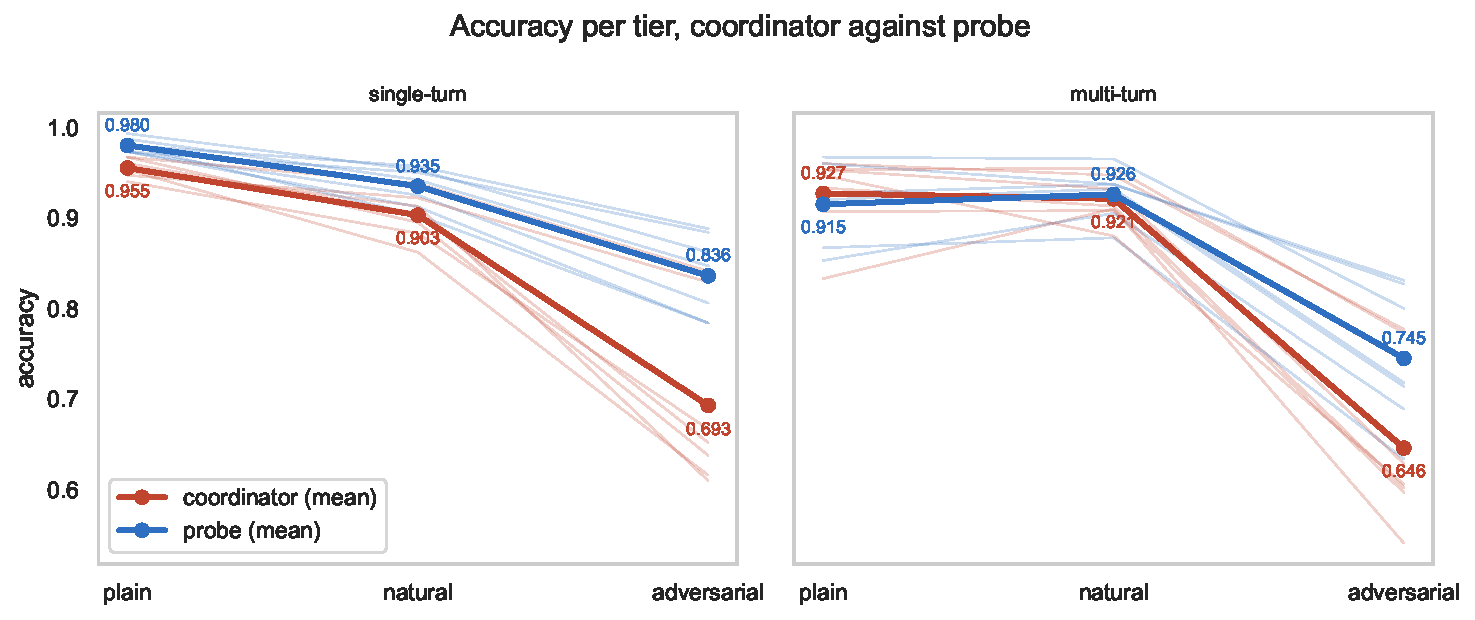
\includegraphics[width=\textwidth]{images/plots/overview/overview_tiers.pdf}
    \caption[Coordinator and probe accuracy across difficulty tiers]{Accuracy of the coordinator and of the probe on each difficulty tier, one panel per dataset. Thick lines are the mean over the seven models, thin lines are single runs. The tier drop is the fall of a line from \texttt{plain} to \texttt{adversarial}.}
    \label{fig:ch8-tiers}
\end{figure}
\FloatBarrier

The mean tier drop of the probe is 0.144 on the single-turn dataset and 0.170 on the multi-turn dataset, against 0.262 and 0.281 for the coordinator. The probe therefore loses less accuracy than the coordinator as the tier becomes harder, and the mean margin is largest on \texttt{adversarial}, 0.143 on the single-turn dataset and 0.099 on the multi-turn dataset. On the single-turn dataset, \texttt{plain} is the easiest tier and \texttt{adversarial} the hardest, for the coordinator and for the probe, in every model.

On the multi-turn dataset, the margin is positive in every model only on \texttt{adversarial}, where its mean is 0.099. On \texttt{plain} the margin is between $-$0.040 and 0.020, and the probe is more accurate than the coordinator in two of the seven models. On \texttt{natural} the margin is between $-$0.030 and 0.048, and the probe is more accurate than the coordinator in three of the seven models. The two tiers are not ordered by difficulty either. The probe is more accurate on \texttt{natural} than on \texttt{plain} in five of the seven models, and the coordinator is more accurate on \texttt{natural} than on \texttt{plain} in three of the seven models. The advantage of the probe on the multi-turn dataset therefore comes from \texttt{adversarial} alone, which holds 900 of the 1650 samples and contributes 0.054 of the mean margin of 0.055.

\FloatBarrier

\subsection{Accuracy Drop on the Multi-Turn Dataset}
\label{subsec:ch8-multi-turn}

The results of Chapter~\ref{chap:probing-results} show that the accuracy of the probe is lower on the multi-turn dataset than on the single-turn dataset for every model. Table~\ref{tab:ch8-multi-turn} reports, per model, the \emph{multi-turn drop} $\Delta_{mt}$ of the coordinator and of the probe, which is the accuracy on the multi-turn dataset minus the accuracy on the single-turn dataset. The table also reports the \emph{drop ratio}, which is the absolute multi-turn drop of the probe divided by the absolute multi-turn drop of the coordinator. The drop ratio is defined only where both multi-turn drops are negative, so it is reported for six of the seven models. The accuracies used to compute both quantities are the ones of Table~\ref{tab:ch8-overview}.

\begin{table}[htbp]
    \centering
    \small
    \begin{tabular}{@{}lccc c ccc c@{}}
        \toprule
        & \multicolumn{3}{c}{\textbf{coordinator accuracy}} & & \multicolumn{3}{c}{\textbf{probe accuracy}} & \\
        \cmidrule(lr){2-4} \cmidrule(lr){6-8}
        \textbf{Model} & \textbf{\begin{tabular}[b]{@{}c@{}}single-\\turn\end{tabular}} & \textbf{\begin{tabular}[b]{@{}c@{}}multi-\\turn\end{tabular}} & $\boldsymbol{\Delta_{mt}}$ & & \textbf{\begin{tabular}[b]{@{}c@{}}single-\\turn\end{tabular}} & \textbf{\begin{tabular}[b]{@{}c@{}}multi-\\turn\end{tabular}} & $\boldsymbol{\Delta_{mt}}$ & \textbf{\begin{tabular}[b]{@{}c@{}}drop\\ratio\end{tabular}} \\
        \midrule
        \texttt{gemma4-e2b-it}     & 0.736 & 0.702 & $-$0.034 & & 0.848 & 0.782 & $-$0.066 & 1.94 \\
        \texttt{qwen3-4b}          & 0.752 & 0.745 & $-$0.007 & & 0.864 & 0.814 & $-$0.050 & 7.14 \\
        \texttt{qwen3-8b}          & 0.772 & 0.738 & $-$0.034 & & 0.845 & 0.744 & $-$0.101 & 2.97 \\
        \texttt{gemma4-12b-it}     & 0.873 & 0.855 & $-$0.018 & & 0.916 & 0.879 & $-$0.037 & 2.06 \\
        \texttt{gemma4-26b-a4b-it} & 0.888 & 0.856 & $-$0.032 & & 0.921 & 0.878 & $-$0.043 & 1.34 \\
        \texttt{llama3.3-70b}      & 0.770 & 0.736 & $-$0.034 & & 0.894 & 0.810 & $-$0.084 & 2.47 \\
        \texttt{qwen2.5-72b}       & 0.761 & 0.768 & $+$0.007 & & 0.907 & 0.875 & $-$0.032 & N/A \\
        \bottomrule
    \end{tabular}
    \caption[Coordinator and probe accuracy across turns, with $\Delta_{mt}$]{Accuracy of the coordinator and of the probe on the single-turn and the multi-turn dataset, with the multi-turn drop $\Delta_{mt}$ and the drop ratio.}
    \label{tab:ch8-multi-turn}
\end{table}

Averaged over the seven models, the multi-turn drop is $-$0.022 for the coordinator and $-$0.059 for the probe. The multi-turn drop of the probe is larger in absolute value than the multi-turn drop of the coordinator in all seven models, including Qwen3 4B and Qwen2.5 72B, where the multi-turn drop of the coordinator accuracy is $-$0.007 and $+$0.007 but the multi-turn drop of the probe accuracy is $-$0.050 and $-$0.032. The drop ratio of Qwen2.5 72B is not defined, because its multi-turn drop of the coordinator is positive: the coordinator is more accurate on the multi-turn dataset than on the single-turn dataset, so the condition for the drop ratio, that both drops be negative, does not hold.

Figure~\ref{fig:ch8-multi-turn} draws the multi-turn drop $\Delta_{mt}$ of Table~\ref{tab:ch8-multi-turn} as one bar for the coordinator and one bar for the probe, per model.

\begin{figure}[htbp]
    \centering
    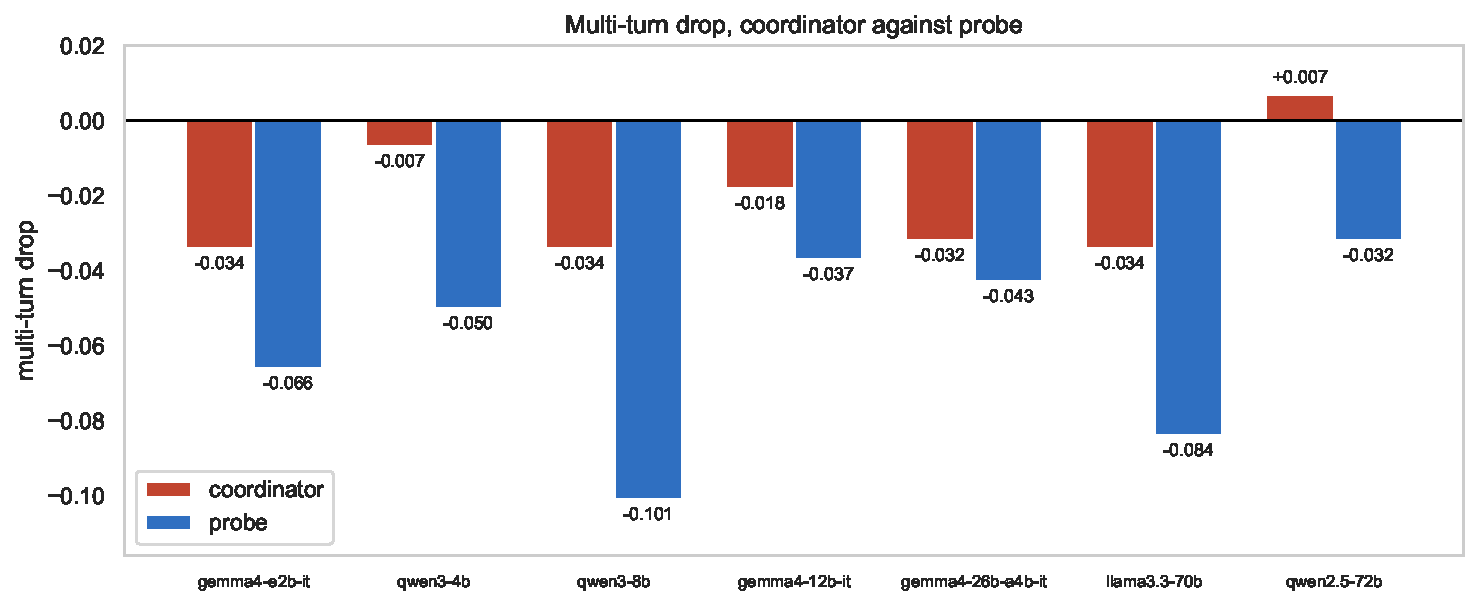
\includegraphics[width=\textwidth]{images/plots/overview/overview_multi_turn.pdf}
    \caption[Multi-turn drop $\Delta_{mt}$ of the coordinator and of the probe, per model]{Multi-turn drop $\Delta_{mt}$ of the coordinator and of the probe, per model. A bar below zero is a lower accuracy on the multi-turn dataset than on the single-turn dataset.}
    \label{fig:ch8-multi-turn}
\end{figure}

\FloatBarrier

\subsection{Answer to RQ1}
\label{subsec:ch8-rq1-answer}

\phantomsection\label{rq:ch8-rq1}
\begin{rqbox}[RQ1]
On requests where the correct sub-agent is difficult to determine from the wording alone, does a probe on the hidden states of a coordinator model recover the correct sub-agent more accurately than the coordinator's own selection?
\end{rqbox}


\noindent Yes. On both datasets and on every model of this section (GPT-OSS 20B excluded), the accuracy of the probe exceeds the accuracy of the coordinator, and the difference is significant in all the runs except Qwen3 8B on the multi-turn dataset, where the margin is 0.006. The mean margin is 0.092 on the single-turn dataset and 0.055 on the multi-turn dataset.

The advantage is largest on the \texttt{adversarial} tier, which is the difficulty tier where the correct sub-agent is the most difficult to determine from the wording of the request. On the single-turn dataset the mean margin grows from 0.025 on \texttt{plain} and 0.032 on \texttt{natural} to 0.143 on \texttt{adversarial}, and on the multi-turn dataset it grows from $-$0.012 and 0.005 to 0.099.

Every tier margin is lower in the multi-turn setting. The multi-turn drop $\Delta_{mt}$ of the probe is larger than the multi-turn drop of the coordinator in all seven models, $-$0.059 against $-$0.022 on average. A possible reason is that, in the multi-turn setting, the hidden state at the last prompt token provides a less separable representation of the sub-agents to train the probe on. Wu et al. report a similar loss of reliability while steering tool selection (adding a direction to the hidden state to change the tool the model calls): the effect becomes inconsistent once the conversation spans several turns \cite{wuToolCallingLinearly2026}.

\FloatBarrier
